\documentclass[11pt, a4paper]{article}

\usepackage[margin=1in]{geometry}
\usepackage{graphicx}
\usepackage{amsmath, amssymb}
\usepackage{listings}
\usepackage{xcolor}
\usepackage{hyperref}
\usepackage{booktabs}
\usepackage{subcaption}
\usepackage{float}
\usepackage{fancyhdr}
\usepackage{enumitem}

\pagestyle{fancy}
\fancyhf{}
\fancyfoot[C]{\thepage}

\begin{document}

\fancypagestyle{no_hdr_border_rule}{
  \renewcommand{\headrulewidth}{0pt}
}
\thispagestyle{no_hdr_border_rule}

\begin{center}
    {\Large \textbf{Experiment 6 -- Report}} \\[0.2cm]
    {\large \textbf{Digital Systems and Microcontrollers (DSM)}} \\[0.1cm]
    {\normalsize International Institute of Information Technology, Hyderabad} \\[0.3cm]
\end{center}

\vspace{0.2cm}
\hrule
\vspace{0.4cm}

\noindent \textbf{Student Name 1:} \textbf{Manbir Singh Judge} \hfill \textbf{Roll Number:} \textbf{2026113005} \\
\noindent \textbf{Student Name 2:} Charishma Kandregula \hfill \textbf{Roll Number:} 2026112022 \\
\noindent \textbf{Table Number:} 16 \hfill \textbf{Lab Room Number:} N114 \\
\noindent \textbf{Date of Experiment:} 09/10/2026

\vspace{0.4cm}
\hrule
\vspace{0.5cm}

\vspace{1em}

\tableofcontents
\vspace{0.5cm}
\hrule
\vspace{0.8cm}

\newpage
\fancyhead[L]{Experiment -- Report}

\fancyhead[R]{Experiment 7}

\section{Aim}
To design and implement a serial adder.

\section{Components \& Equipment Required}
\begin{itemize}
    \item Digital Test Kit (DTK) -- including power supply, switches, indicator LED pairs and breadboard
    \item \textbf{ICs}: CD40xx series for NAND, NOR and XOR gates
    \item Connecting Wires
\end{itemize}

\section{Procedure}

\subsection{Design}
\begin{enumerate}[label=\arabic*., font=\bfseries]
    \item \textbf{High-level design of Serial Adder:}
    \begin{itemize}
        \item We require the adder to add a series of bits one-by-one starting from LSB. That requires storing the carry from previous addition.
        \item To achieve this, we can use a D flip-flop connected to output of the full-adder. And, its output is connected to input carry of the full-adder.
        \item This the resulting block diagram:
        \begin{figure}[H]
            \centering
            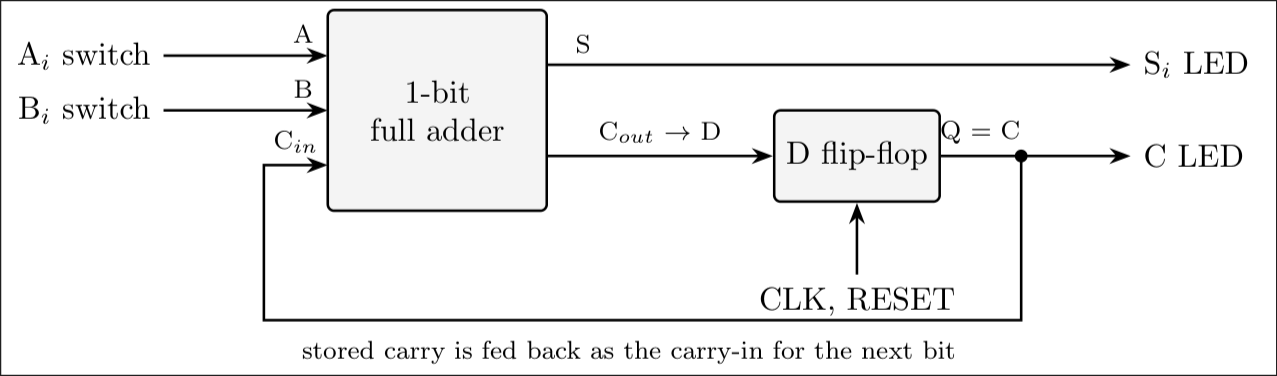
\includegraphics[width=0.8\textwidth]{block-dgm_seial-adder.png}
            \caption{Block Diagram for Serial Adder}
        \end{figure}
    \end{itemize}
    \item \textbf{Design of Full-Adder (FA):}
    \begin{itemize}
        \item We know $S = A \oplus B \oplus C_{in}$ and $C_{out} = AB + (A \oplus B)C_{in}$.
        \item To avoid usage of OR gate, we can generate the signals as follows:
        \begin{itemize}[label=$\circ$]
            \item $S_1 = A \oplus B$
            \item $S = S_1 \oplus C_{in}$
            \item $X = \overline{AB}$
            \item $Y = \overline{S_1 C_{in}}$
            \item $C_{out} = \overline{XY}$
        \end{itemize}
        % \item Resulting circuit:
        % \begin{figure}[H]
        %     \centering
        %     \includegraphics[width=0.34\textwidth]{circuit_fa.png}
        %     \caption{Circuit for Full Adder}
        % \end{figure}
    \end{itemize}
    \item \textbf{Design of D Flip-Flop (D-FF):}
    \begin{itemize}
        \item We already know design of D-FF with a clear signal:
        \begin{figure}[H]
            \centering
            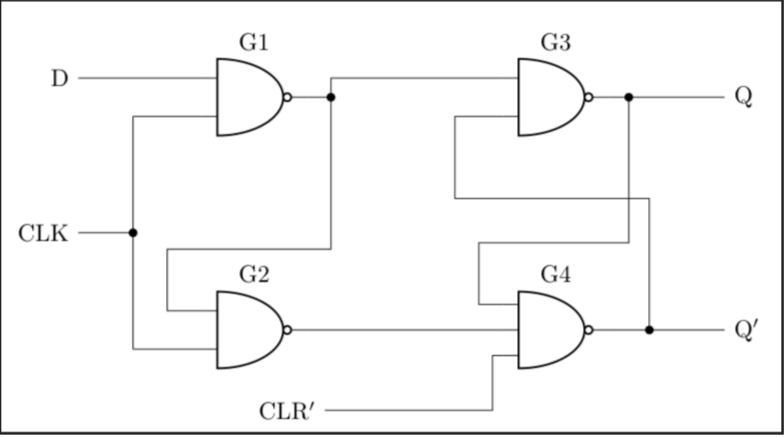
\includegraphics[width=0.6\textwidth]{circuit_dff.png}
            \caption{Circuit Diagram of D Flip-Flop}
        \end{figure}
    \end{itemize}
\end{enumerate}

\subsection{Implementation and Observation}
\begin{itemize}
    \item Implement the designed circuit in Tinkercad. Verify it works for the following input:
        $$0110 + 0111 = 0\_1101$$
    \item Place the required ICs on the breadboard and verify the operation of each gate.
    \item Wire the circuit according to the designed circuit diagrams using gates from above ICs.
    \item Use the same inputs (used to test Tinkercad) to test our hardware circuit. Record the serial output and final carry.
\end{itemize}

\section{Observations}
Serial input 1, $A = 0110$ \newline
Serial input 2, $B = 0111$ \newline
Serial output, $S = 1101$ \newline
Final carry out, $C_{out} = 0$ \newline

\section{Tinkercad Simulation}
\noindent \textbf{Tinkercad Link:} \href{https://www.tinkercad.com/things/akDqqkdBcv7-dsm-experiment-6?sharecode=bZbyLLDM4noThxqIrUkIJUBuu61gs2dZgRE7n2ZMN0A}{\color{blue}Click here}
\begin{figure}[H]
\centering
    \centering
    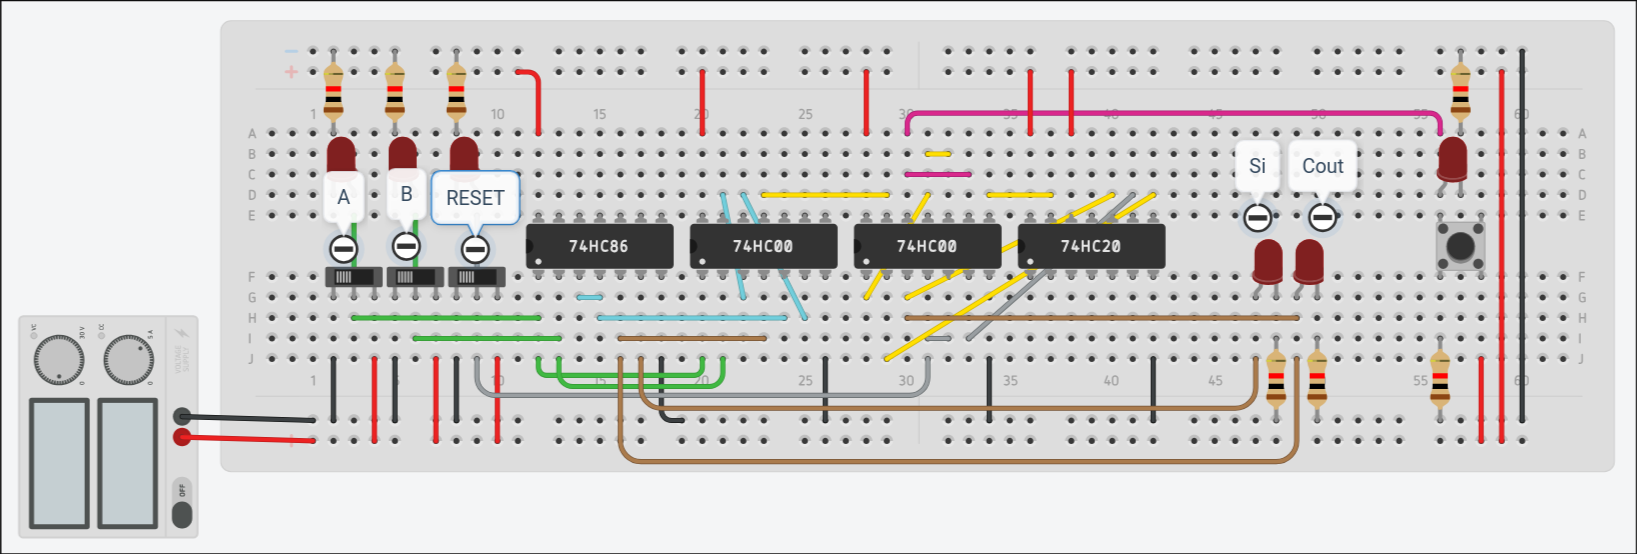
\includegraphics[width=\textwidth]{tc.png}
    \caption{Tinkercad Simulation Screenshot}
\end{figure}

\section{Hardware Setup Photograph}
\begin{figure}[H]
    \centering
    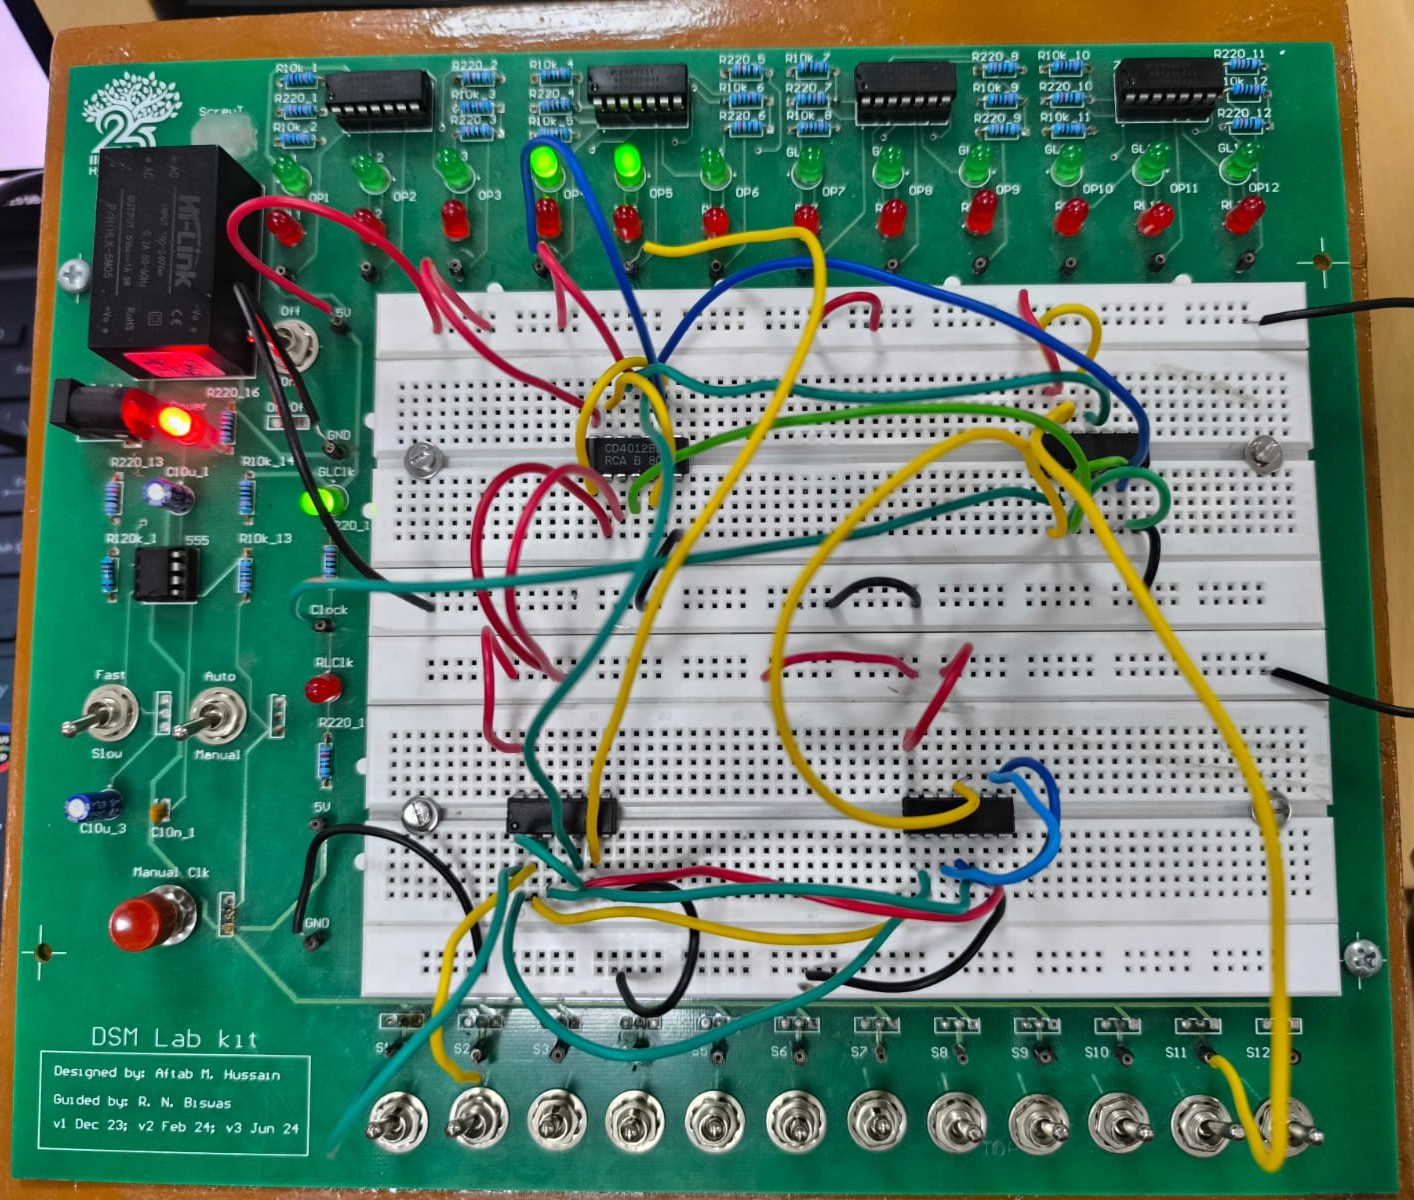
\includegraphics[width=0.8\textwidth]{lab.jpeg}
    \caption{Hardware Circuit for Serial Adder}
\end{figure}

\section{Conclusion}
A 1-bit serial adder was designed, implemented and tested.

\end{document}